\documentclass[12pt]{article}

\usepackage{sbc-template}
\usepackage[brazil,american]{babel}
\usepackage[utf8]{inputenc}

\usepackage{graphicx}
\usepackage{url}
\usepackage{float}
\usepackage{listings}
\usepackage{color}
\usepackage{todonotes}
\usepackage{algorithmic}
\usepackage{algorithm}
\usepackage{hyperref}
\usepackage{amssymb}
\usepackage{amsmath}
\graphicspath{{../parte1/graficos/}{../parte2/graficos/}}

\sloppy

\title{Trabalho 2\\
Ajuste de Curvas\\
\& \\
Splines}

\author{Dayanne Fernandes da Cunha, 13/0107191\\
       Yurick Hauschild, 12/0024136\\
       Grupo 6
}

\address{Dep. Matemática $-$ Universidade de Brasília (UnB)\\
  Cálculo Numérico $-$ Turma A
  \email{dayannefernandesc@gmail.com, yurick.hauschild@gmail.com}
}

\begin{document}
\maketitle

\selectlanguage{brazil}

 \begin{resumo}
 	Este relatório corresponde aos informativos das resoluções do Trabalho 2 de Cálculo Numérico da Turma A do semestre 2016/2.
 \end{resumo}

\section{Parte I : Ajuste de Curvas}
\label{sec:parte1}

Esta primeira parte de trabalho será dedicada ao ajustes de curvas pelo método dos mínimos quadrados. Para tal, considere o conjunto de dados apresentado na Figura~\ref{fig:tab1}.

\begin{figure}[H]
	\centering
	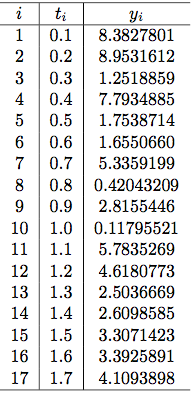
\includegraphics[width=0.3\textwidth]{tab1.png}
	\caption{Tabela de pontos.}
	\label{fig:tab1}
\end{figure}

\subsection{Questão 1}
\label{subsec:p1q1}

Determine, para o conjunto de pontos da Figura~\ref{fig:tab1}, os melhores ajustes polinomiais de grau 1, 2, 3, 5 e 10. Trace os seus resultados e comente sobre a adequação de cada um destes ajustes. É possível encontrar uma maneira quantitativa de se julgar qual dentre estes cinco ajustes é o melhor?

\textbf{Resolução:}


\subsection{Questão 2}
\label{subsec:p1q2}

Encontre o polinômio interpolador para estes dados e trace o seu resultado num gráfico. Apresente, igualmente, o polinômio interpolador encontrado teoricamente, usando polinômios de Lagrange (talvez seja recomendado usar algum programa de manipulação simbólica!). Comente seus resultados. Se você precisasse de uma função para descrever os dados da tabela, qual dentre o polinômio interpolador e os ajustes encontrados na questão 1 você escolheria? Por quê?

\textbf{Resolução:}

Para tentar ajustar os pontos da Figura~\ref{fig:tab1} foi utilizado o método de mínimos quadrados na questão 1, já nesta questão foi requisitado que ajustasse a curva utilizando o polinômio interpolador utilizando polinômios de Lagrange.

Para uma determinada função $f(x)$ se tivermos n+1 pontos $(x_{i}, y_{i})$ com $t_{i} \neq t_{j}$ $\forall i,j$ sempre encontraremos um único polinômio interpolador de grau menor ou igual a $n$ tal que $y(x_{i}) = y_{i} \forall i=1,..,n+1$.

Por propriedade do polinômio interpolador, a de passar exatamente em todos os pontos $(x_{i}, y_{i})$, o erro do ajuste é \textbf{nulo} ($\mathcal{E}\equiv 0$)! 

\begin{figure}[H]
	\centering
	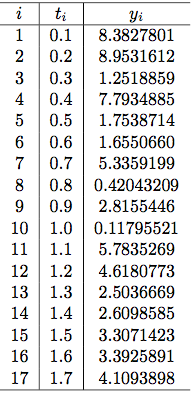
\includegraphics[width=0.3\textwidth]{tab1.png}
	\caption{Tabela de pontos.}
	\label{fig:tab1}
\end{figure}

\subsection{Questão 3}
\label{subsec:p1q3}

\textbf{Resolução:}

\subsection{Questão 4}
\label{subsec:p1q4}

\textbf{Resolução:} 

\section{Parte II : Splines}
\label{sec:parte2}

\subsection{Questão 5}
\label{subsec:p2q5}

\textbf{Resolução:}

\subsection{Questão 6}
\label{subsec:p2q6}

\textbf{Resolução:}

\subsection{Questão 7}
\label{subsec:p2q7}

\textbf{Resolução:}

\subsection{Questão 8}
\label{subsec:p2q8}

\textbf{Resolução:}

\subsection{Questão 9}
\label{subsec:p2q9}

\textbf{Resolução:} 

\end{document}
